\chapter{Frontend}
Bei dem Frontend handelt es sich um den in Java programmierten Client und Server.
Mit Ausnahme der Dateisynchronisation arbeitet es völlig unabhängig vom Backend.
Im Großen und Ganzen werden folgende Aufgaben erfüllt:
\begin{itemize}
	\item Netzwerkkommunikation zwischen den Clients und dem Archivserver.
	\item Programmierschnittstelle für Java-Tools, die das Archiv nutzen wollen.
	\item Benachrichtigung der Nutzer über Änderungen.
\end{itemize}
\section{Use-Cases}
In Use-Case Diagramm \ref{design:dia:usecase} sind alle wesentlichen Ereignisse (Use-Cases) zusammengefasst, die sich im Frontend abspielen.
\subsection{Notifier}
Der Notifier arbeitet als eigenständiger Thread im Server.
\begin{description}
	\item [select]
		Der Notifier führt eigenständig Datenbankabfragen durch,
		um Änderungen zu ermitteln.
	\item [notifyClients und notifyObservers]
		Die Änderungen werden an alle registrierten Clients gesendet.
		Die Clients wiederum geben die Änderungen an angemeldete Observer weiter.
\end{description}

\subsection{Java User}
Java User stellen alle Akteure dar die den Client in ihr Programm einbinden. 

\begin{description}
	\item [initClient und registerClient]
		beim starten des Client meldet sich dieser beim Server und wird dort registriert.
	\item [select]
		über vorbereite sql-select Schnittstellen können MetaDatenobjekte aus der
		Datenbank abgefragt werden.
	\item [getFileList]
		Es wird eine Dateiliste eines \arc-Verzeichnisses zurückgegeben.
	\item [getOutputStream]
		Es wird ein Outputstream zurückgegeben um Dateien in das Archiv zu schreiben.
	\item [getInputStream]
		Über einen Inputstream können aus dem Archiv gelesen werden.
	\item [getXMLData]
		Es werden bestimmte XML-Daten zurückgegeben.
	\item [addXMLData]
		Es können neue Elemente zu den XML-Daten hinzugefügt werden.
	\item [add / deleteObserver]
		Es können Observer an- und abgemeldet werden, welche Update-daten aus dem
		Archiv bekommen können.
\end{description}
\begin{figure}[!h]
	\centering
	\label{design:dia:usecase}
	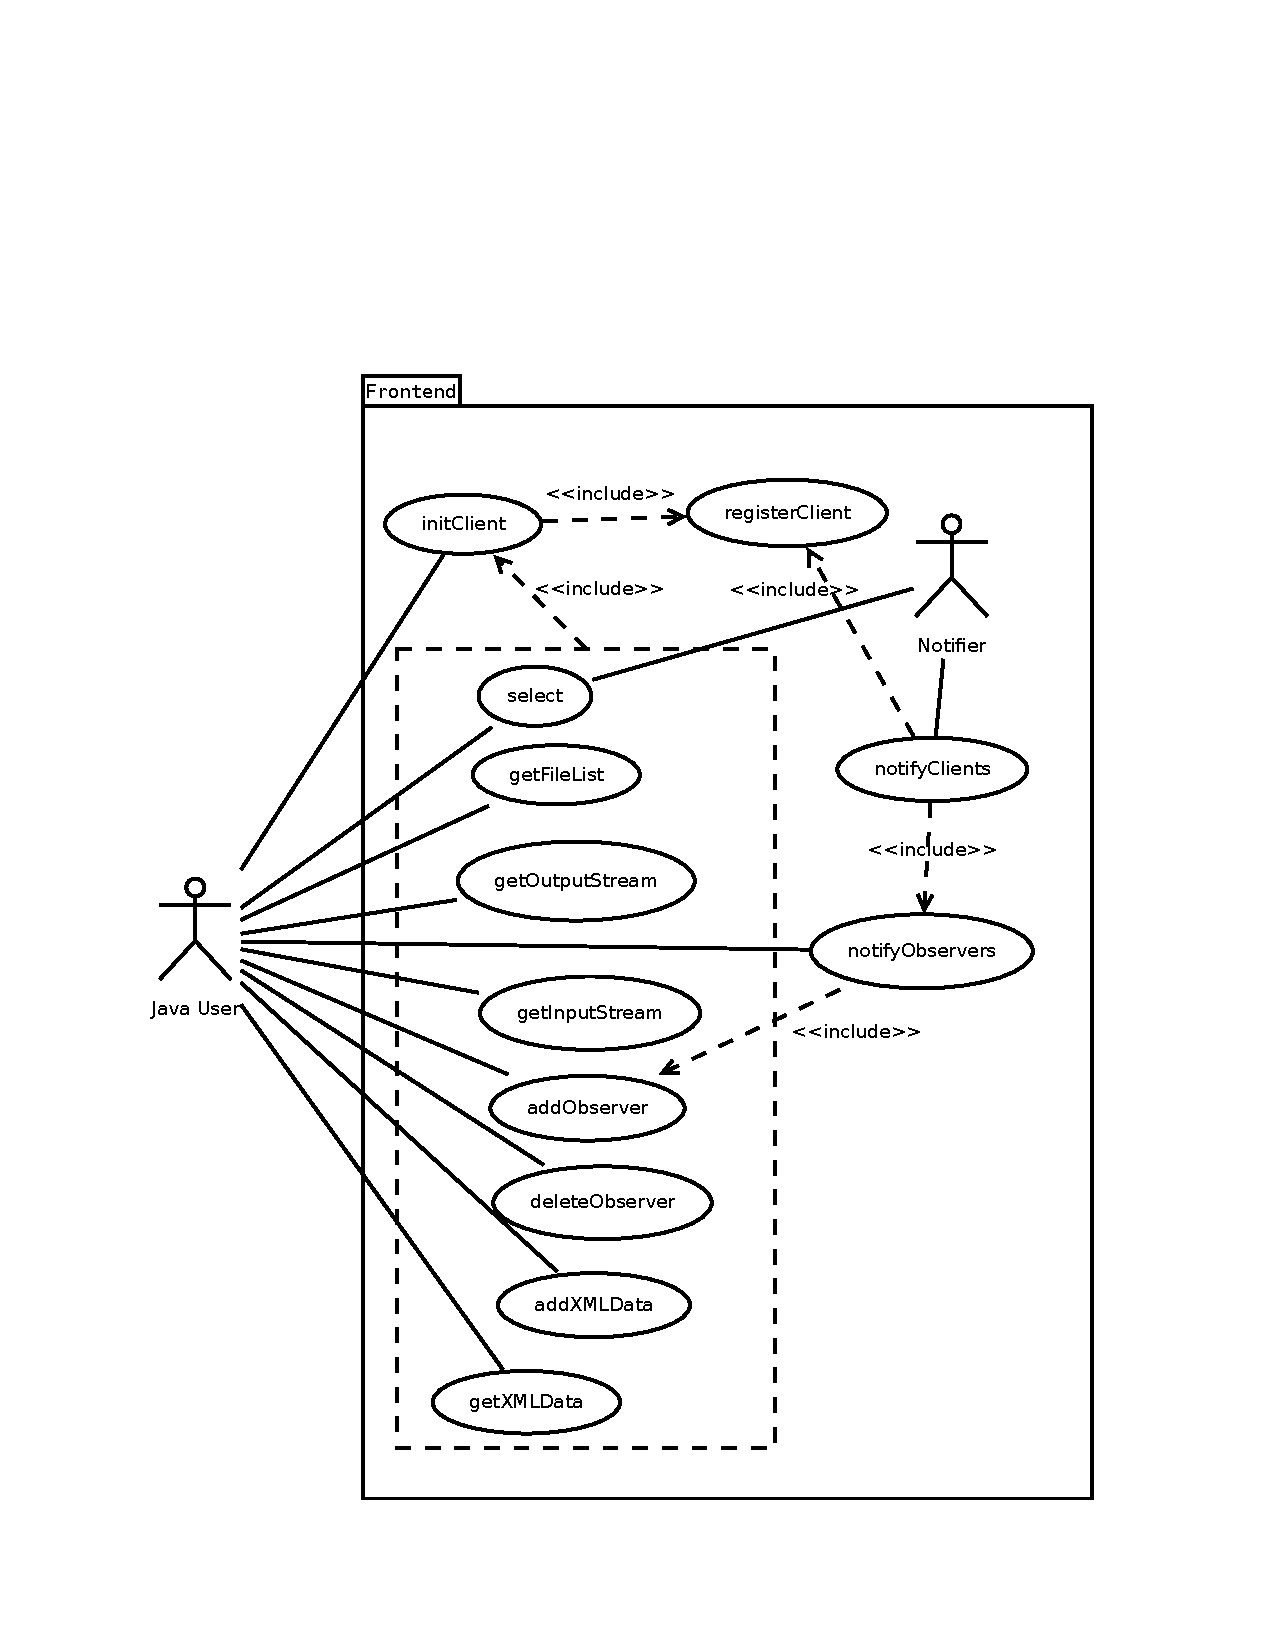
\includegraphics[height=0.9\textheight]{design/frontend/usecase.pdf}
	\caption{Diagramm: Use-Cases - Client und Server}
\end{figure}

\newpage

\section{Schnittstellen und Api}

\section{Programmfluss}

\subsection {select}

\begin{figure}[h]
	\centering
	\label{design:dia:sqc:select}
	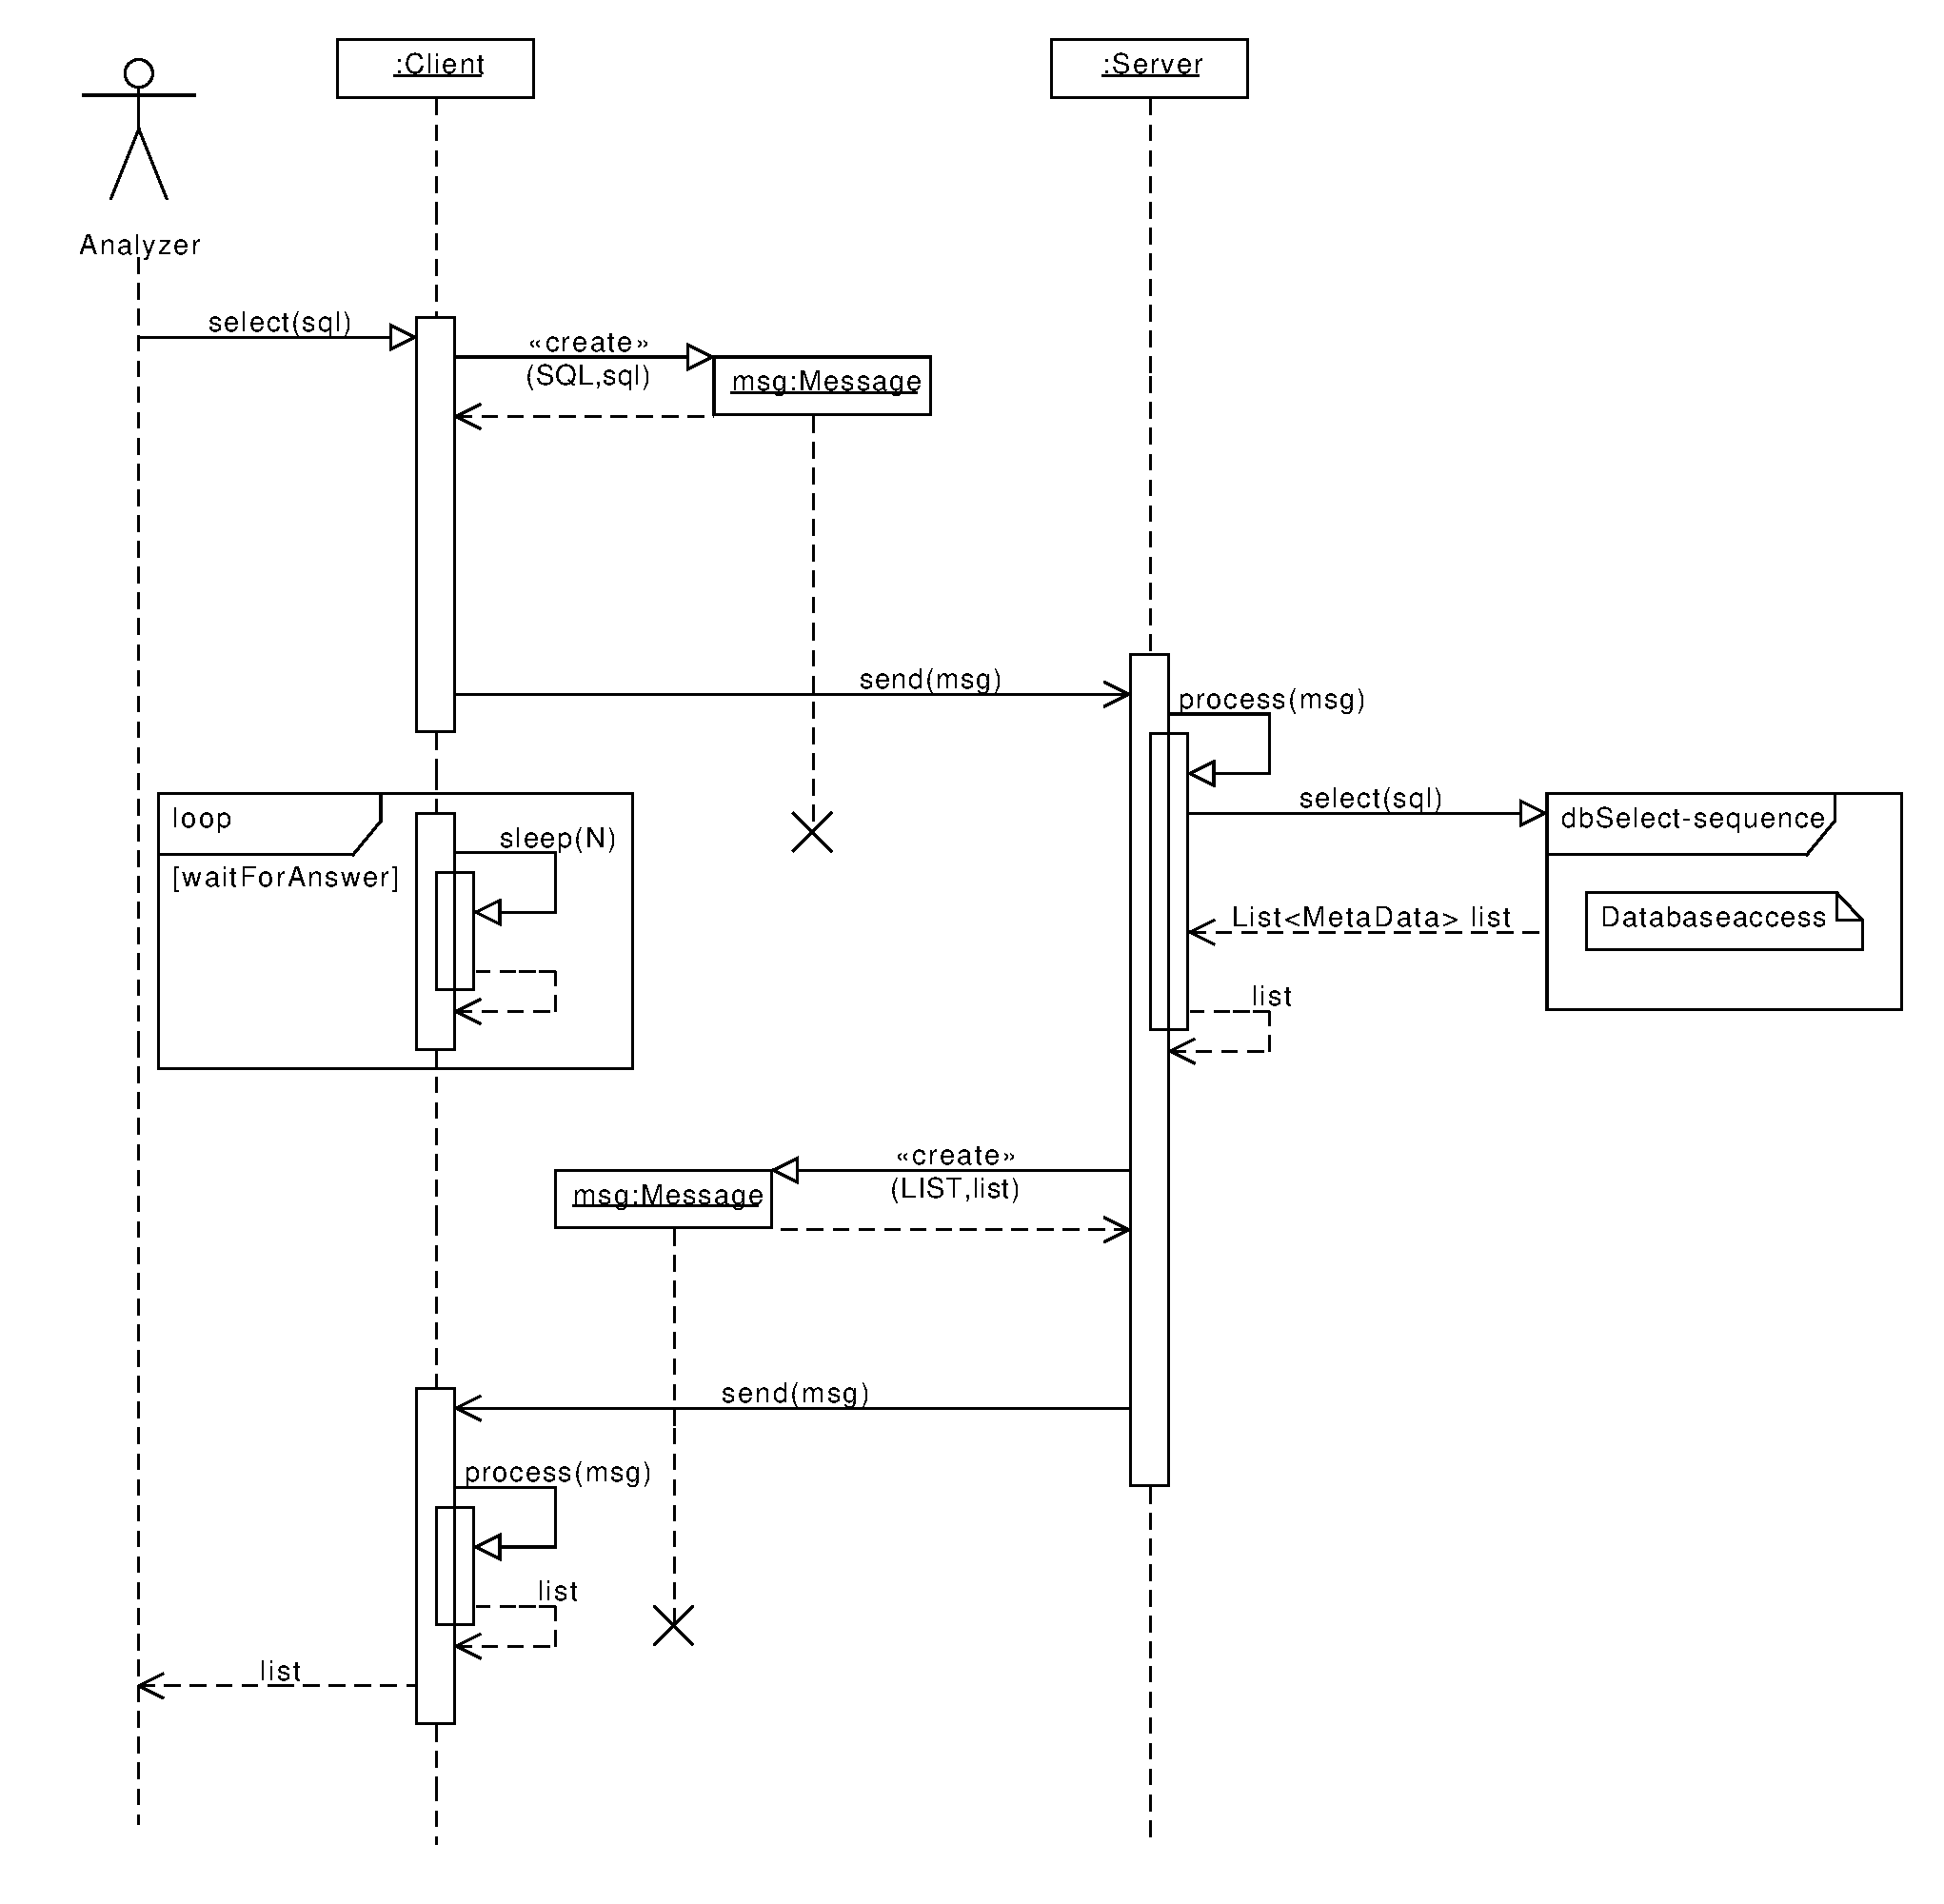
\includegraphics[width=\textwidth]{design/frontend/sequence/select-sequence.pdf}
	\caption{Sequenzdiagramm: Select}
\end{figure}

\subsection {getFileList}
\todo{sequence: getFileList}
%\begin{figure}[h]
%	\centering
%	\label{design:dia:sqc:select}
%	\includegraphics[width=\textwidth]{design/frontend/sequence/.pdf}
%	\caption{Sequenzdiagramm: Select}
%\end{figure}

\subsubsection{Lock setzen}
\begin{figure}[h]
	\centering
	\label{design:dia:sqc:lock}[h]
	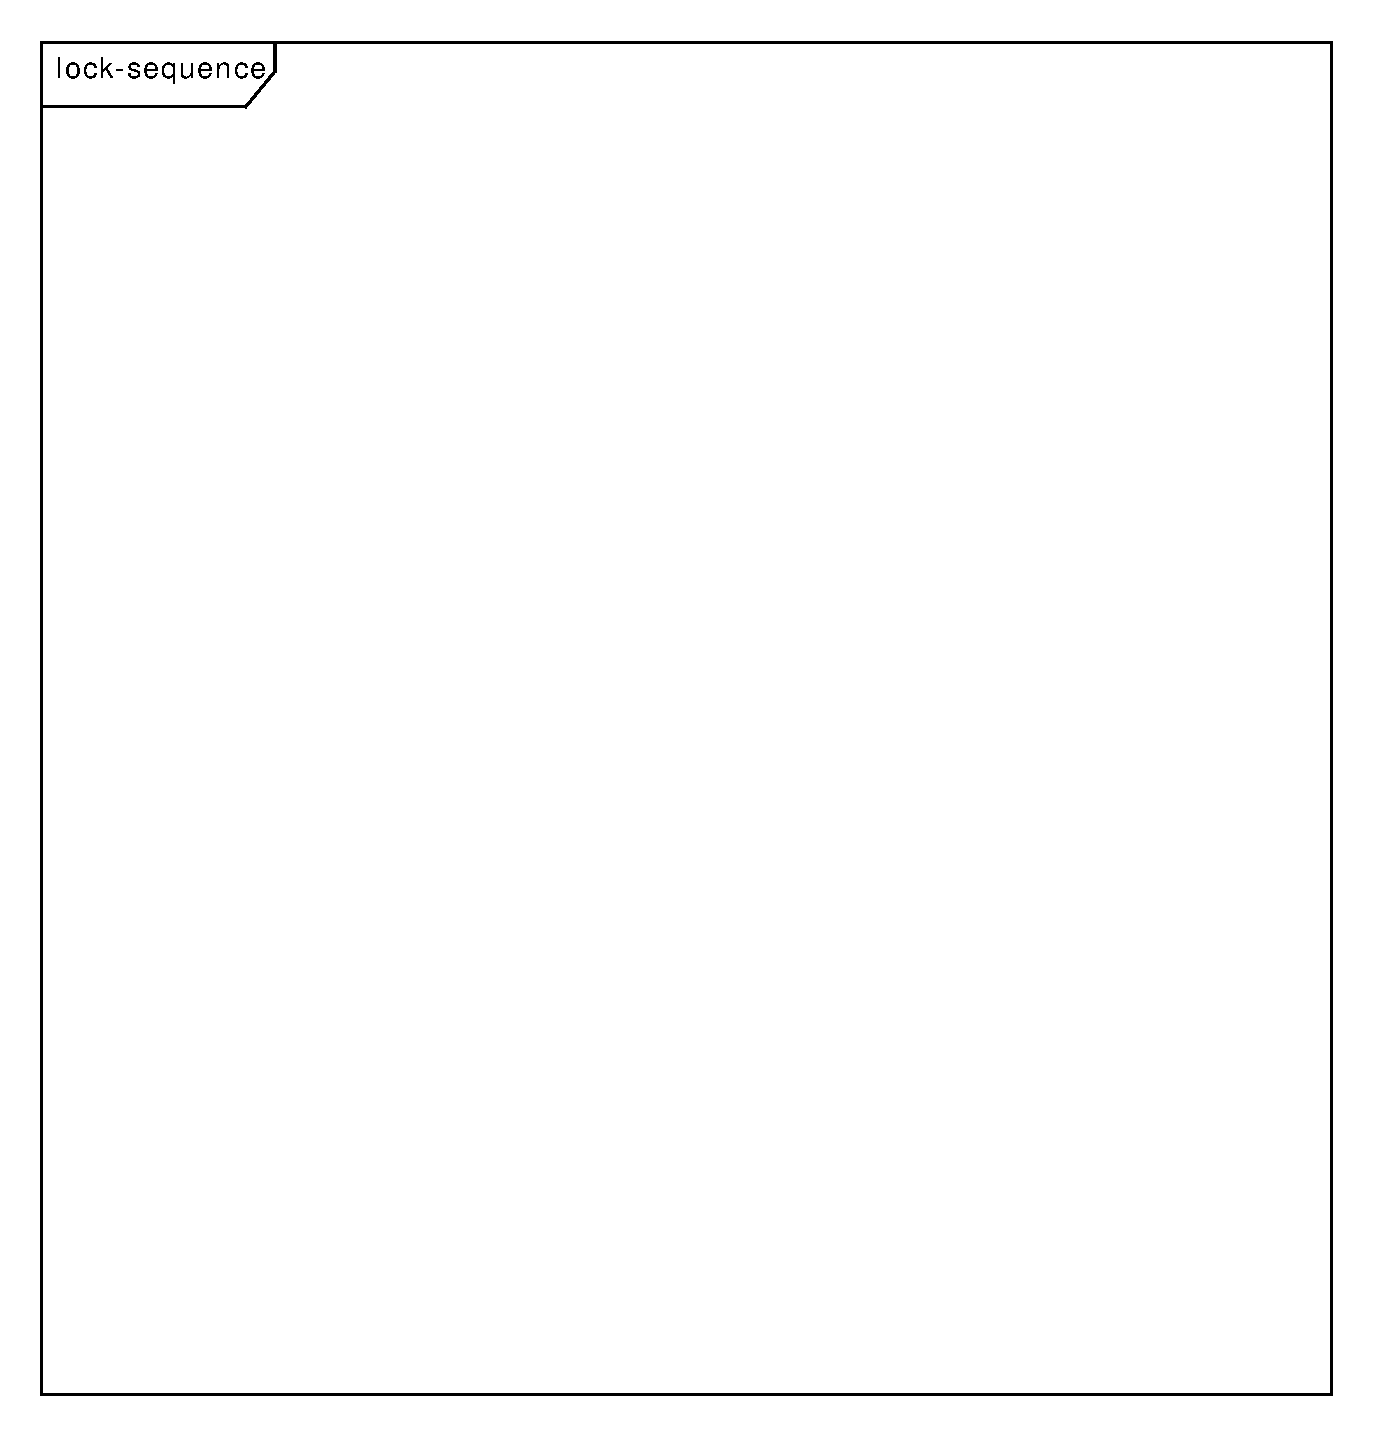
\includegraphics[width=0.5\textwidth]{design/frontend/sequence/lock-sequence.pdf}
	\caption{Sequenzdiagramm: Lock setzen}
\end{figure}

\subsubsection{Unlock}
\begin{figure}[h]
	\centering
	\label{design:dia:sqc:unlock}[h]
	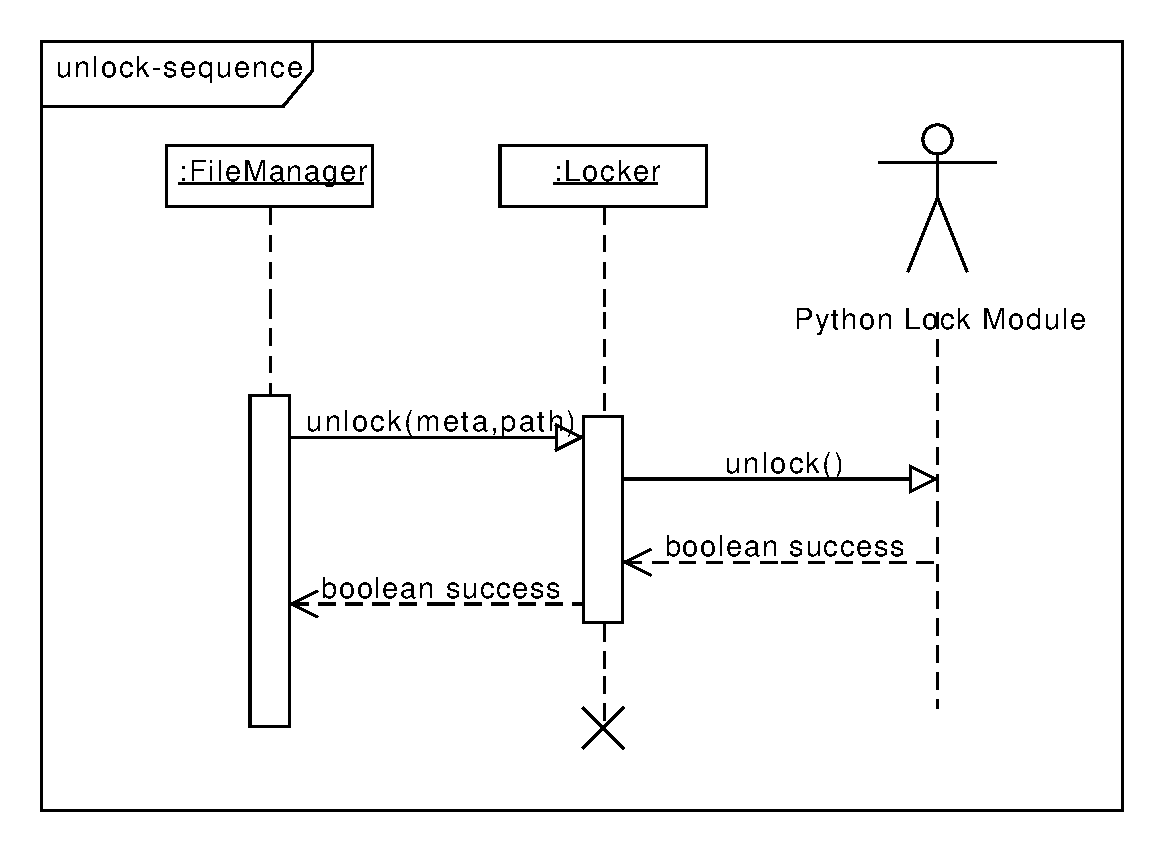
\includegraphics[width=0.5\textwidth]{design/frontend/sequence/unlock-sequence.pdf}
	\caption{Sequenzdiagramm: Unlock}
\end{figure}

\subsection {getOutputStream}
\begin{figure}[h]
	\centering
	\label{design:dia:sqc:getOutputStream}[h]
	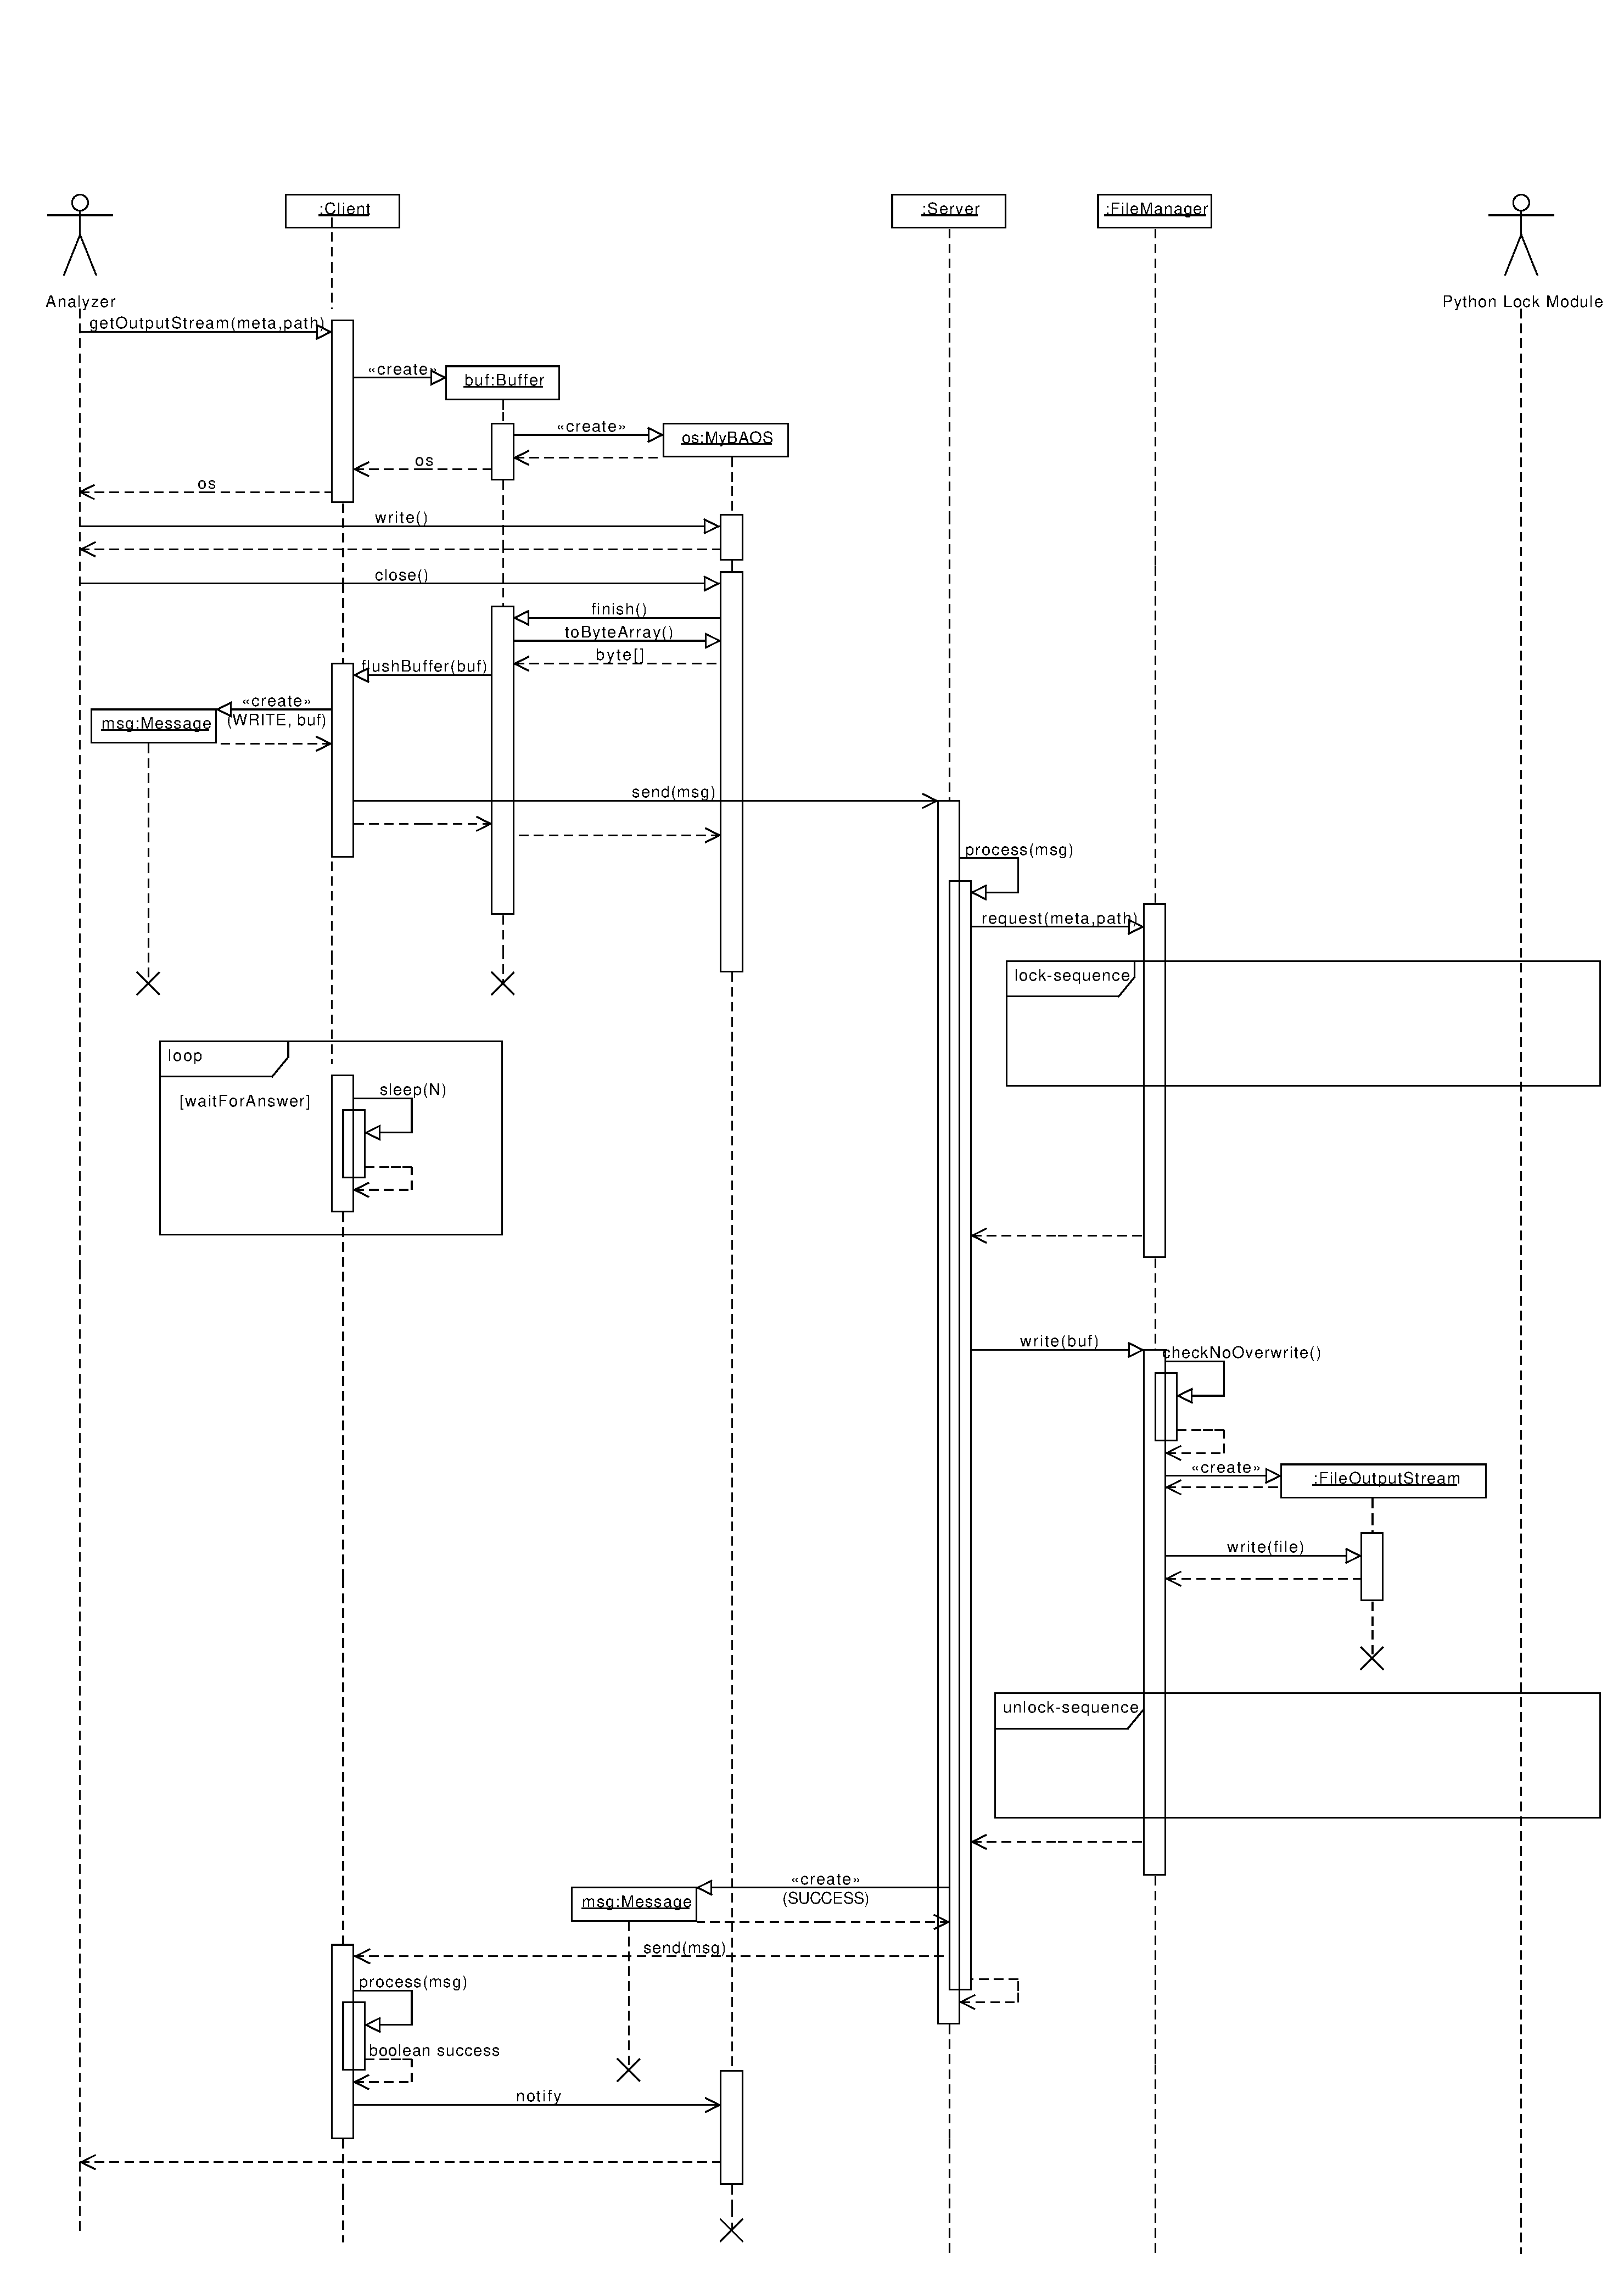
\includegraphics[width=\textwidth]{design/frontend/sequence/get-output-stream-sequence.pdf}
	\caption{Sequenzdiagramm: getOutputStream}
\end{figure}

\subsection {getInputStream}
\begin{figure}[h]
	\centering
	\label{design:dia:sqc:getInputStream}[h]
	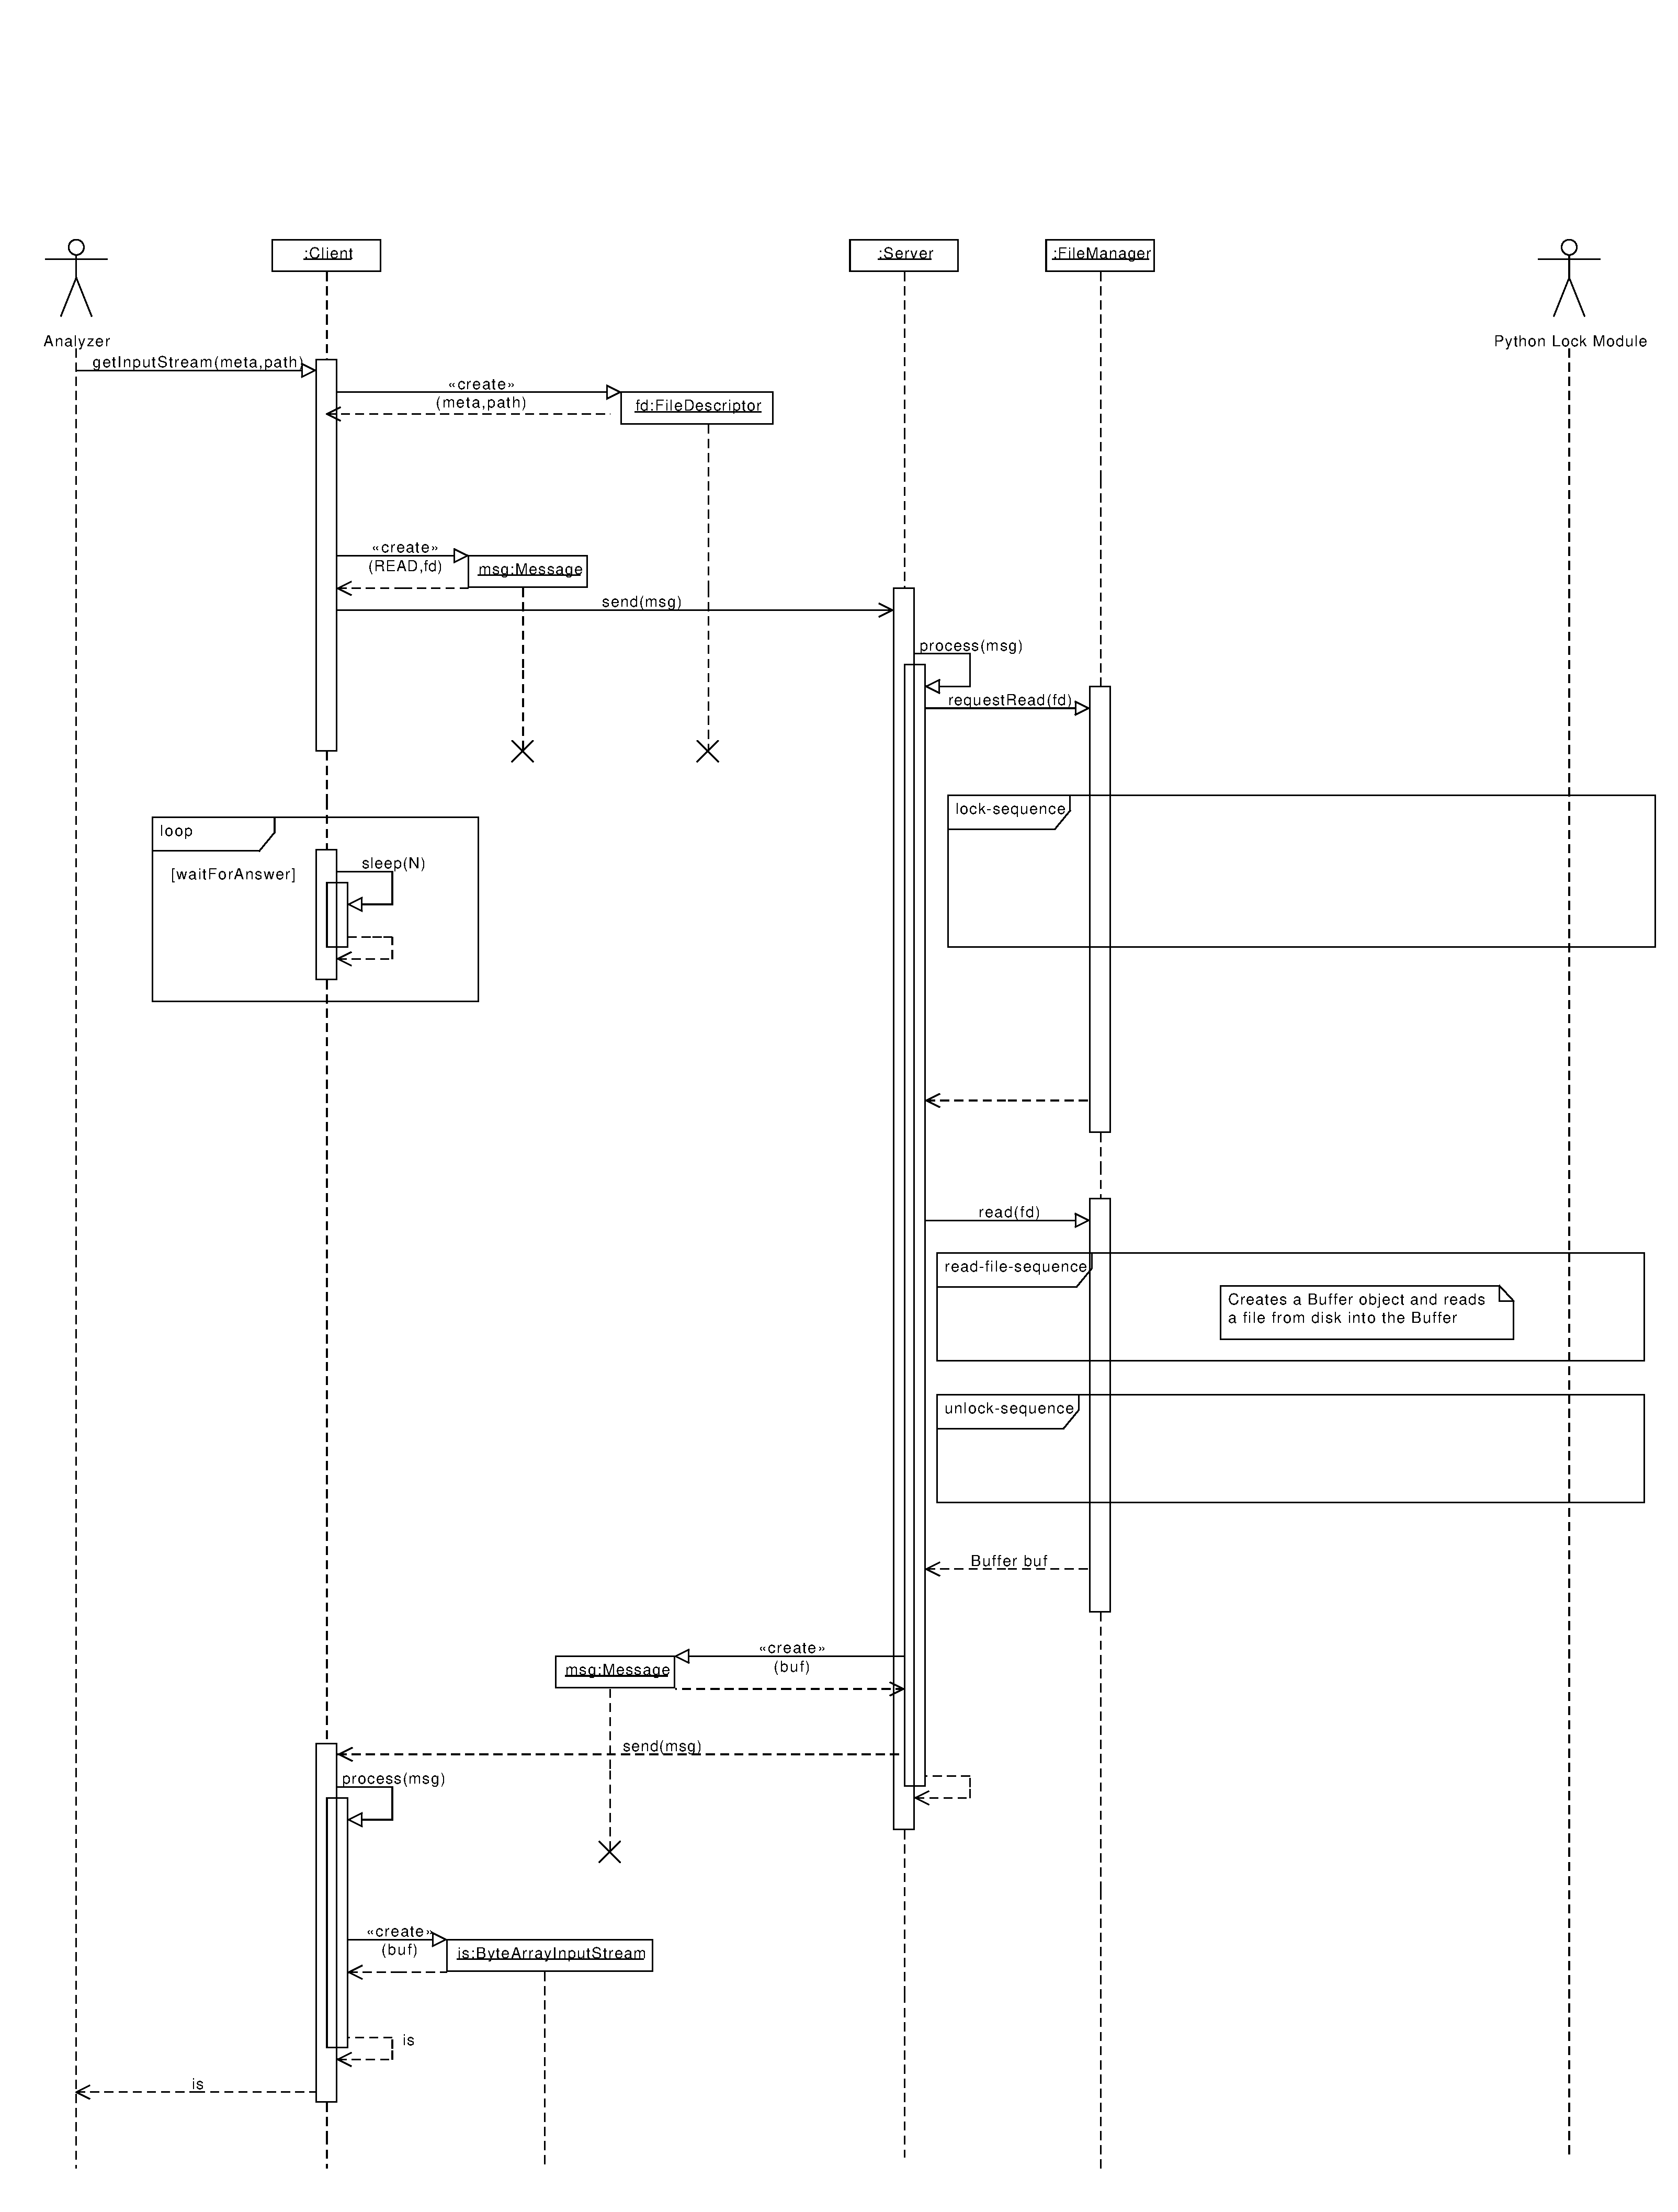
\includegraphics[width=0.5\textwidth]{design/frontend/sequence/get-input-stream-sequence.pdf}
	\caption{Sequenzdiagramm: getInputStream}
\end{figure}

\subsection {getXMLData}
\todo{sequence: getXMLData}
%\begin{figure}[h]
%	\centering
%	\label{design:dia:sqc:select}
%	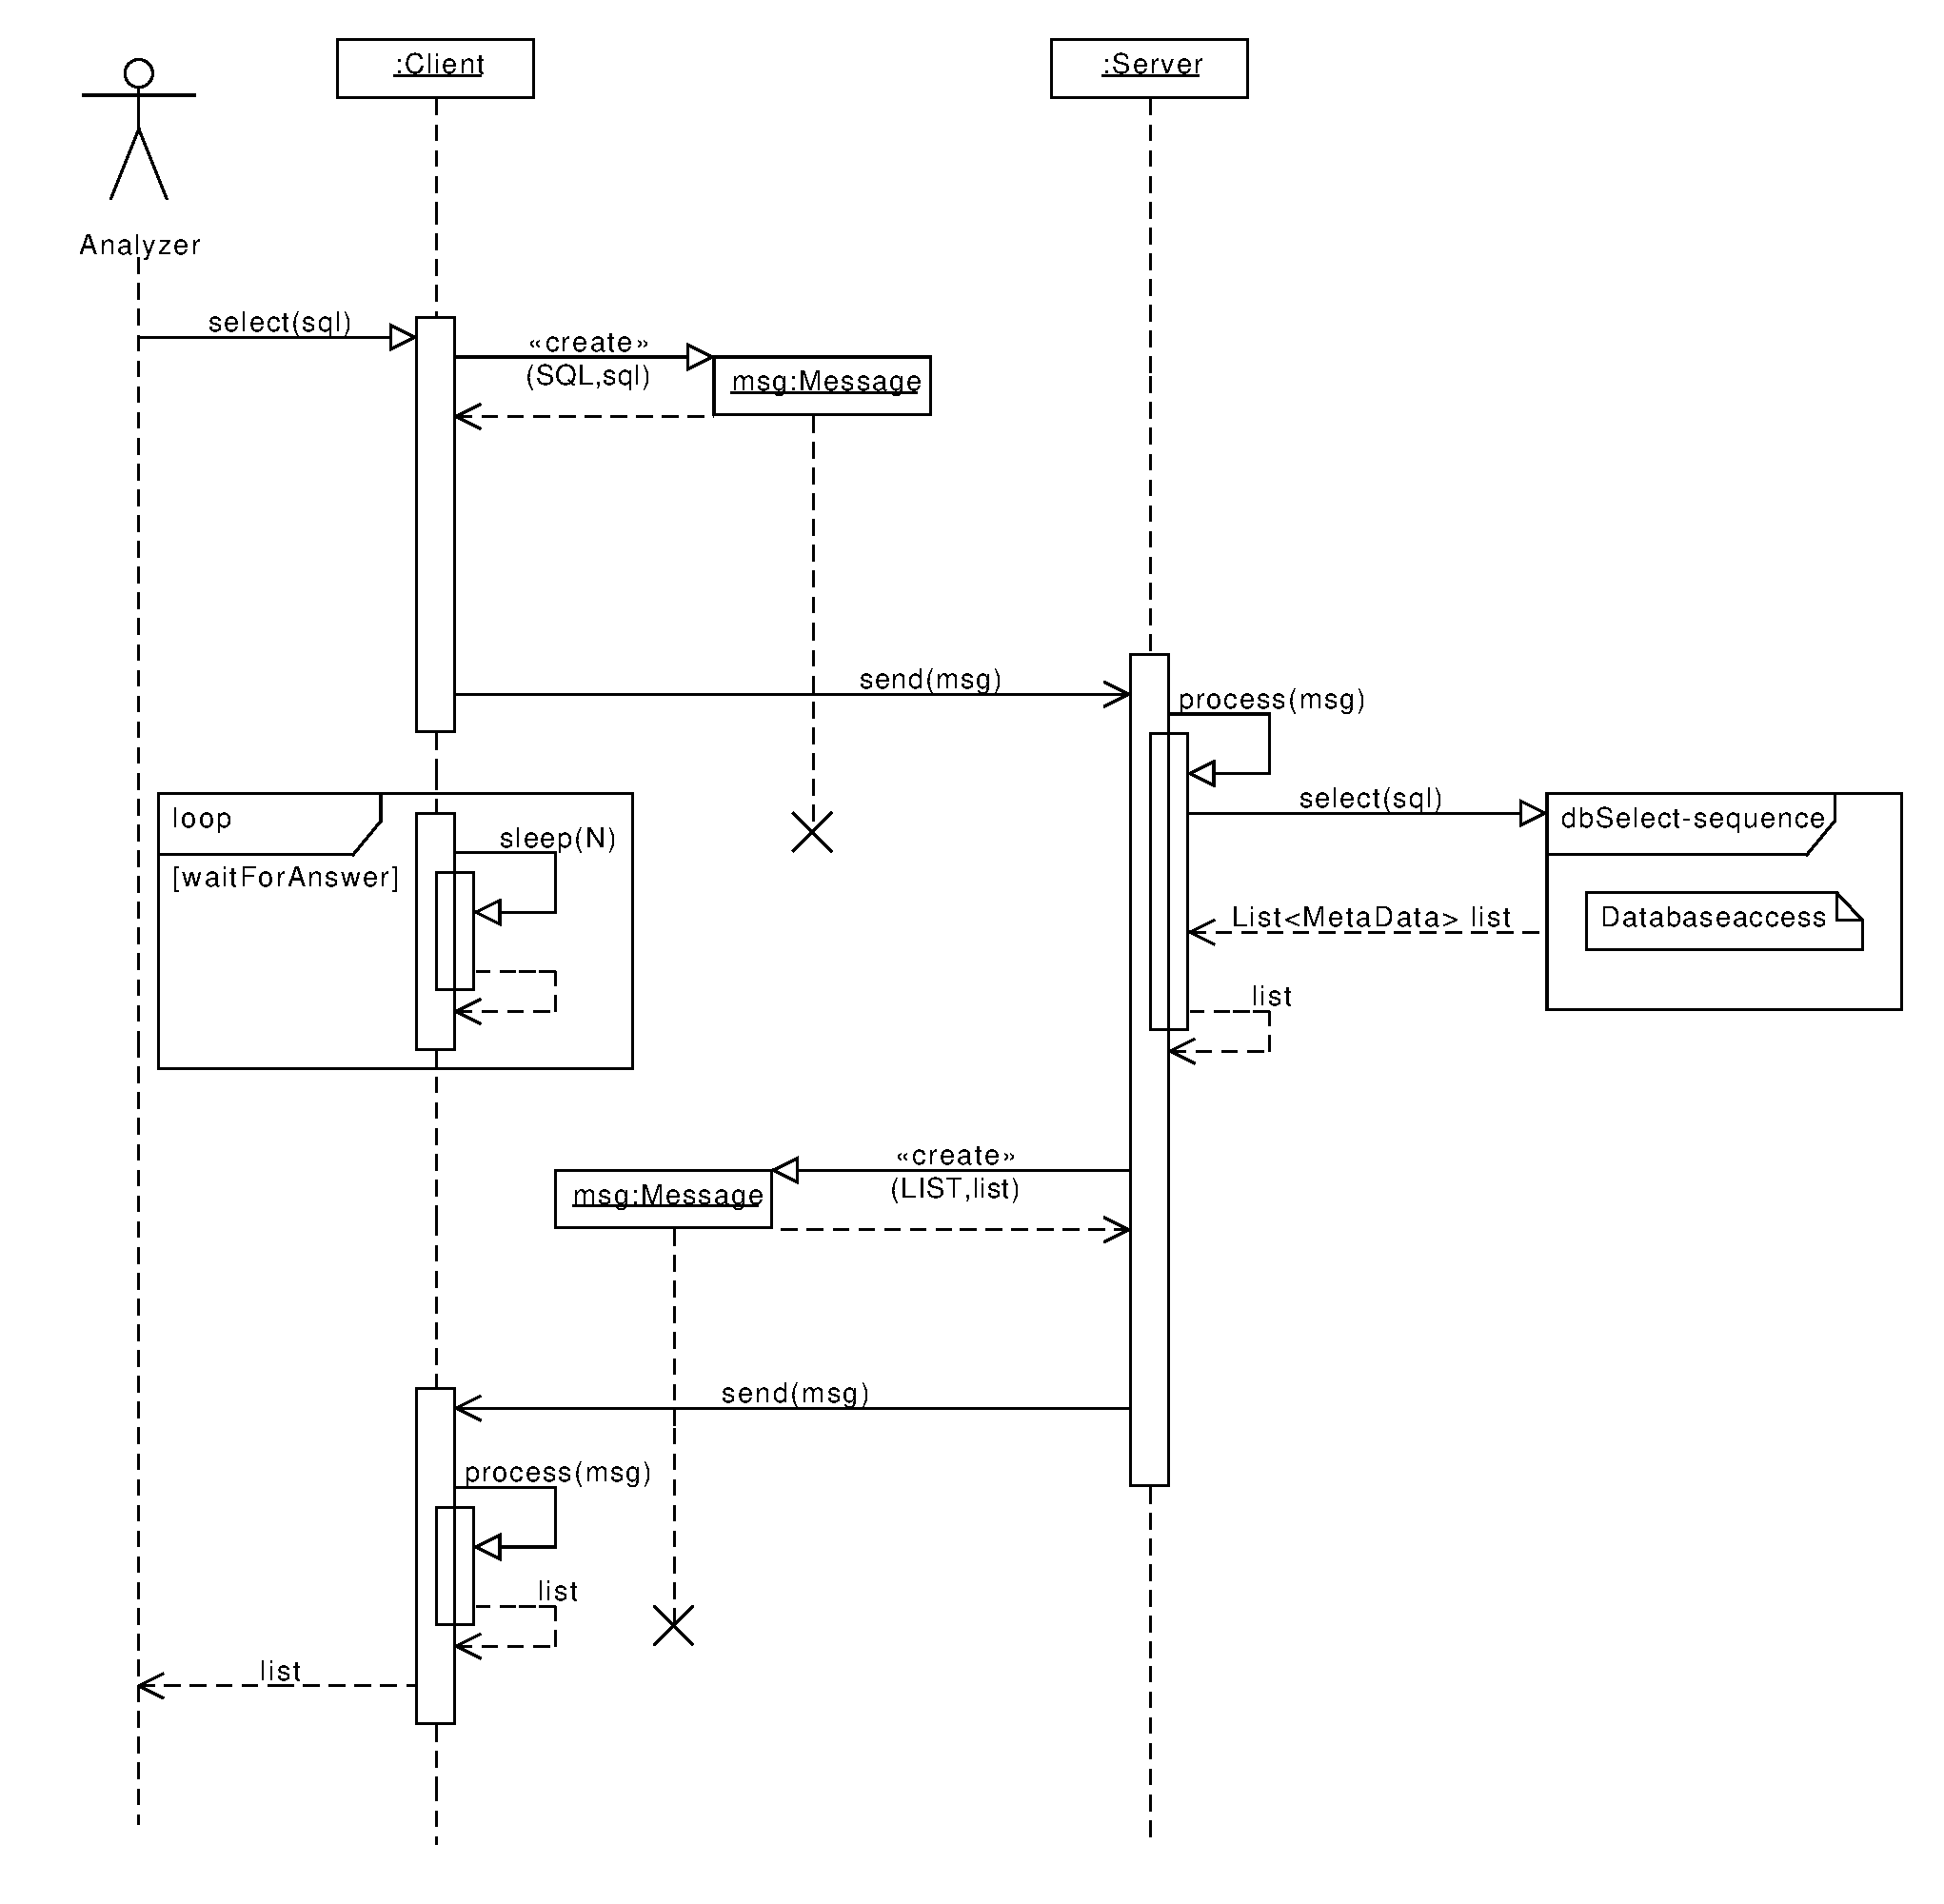
\includegraphics[width=\textwidth]{design/frontend/sequence/select-sequence.pdf}
%	\caption{Sequenzdiagramm: Select}
%\end{figure}

\subsection {addXMLData}
\todo{sequence: addXMLData}
%\begin{figure}[h]
%	\centering
%	\label{design:dia:sqc:select}
%	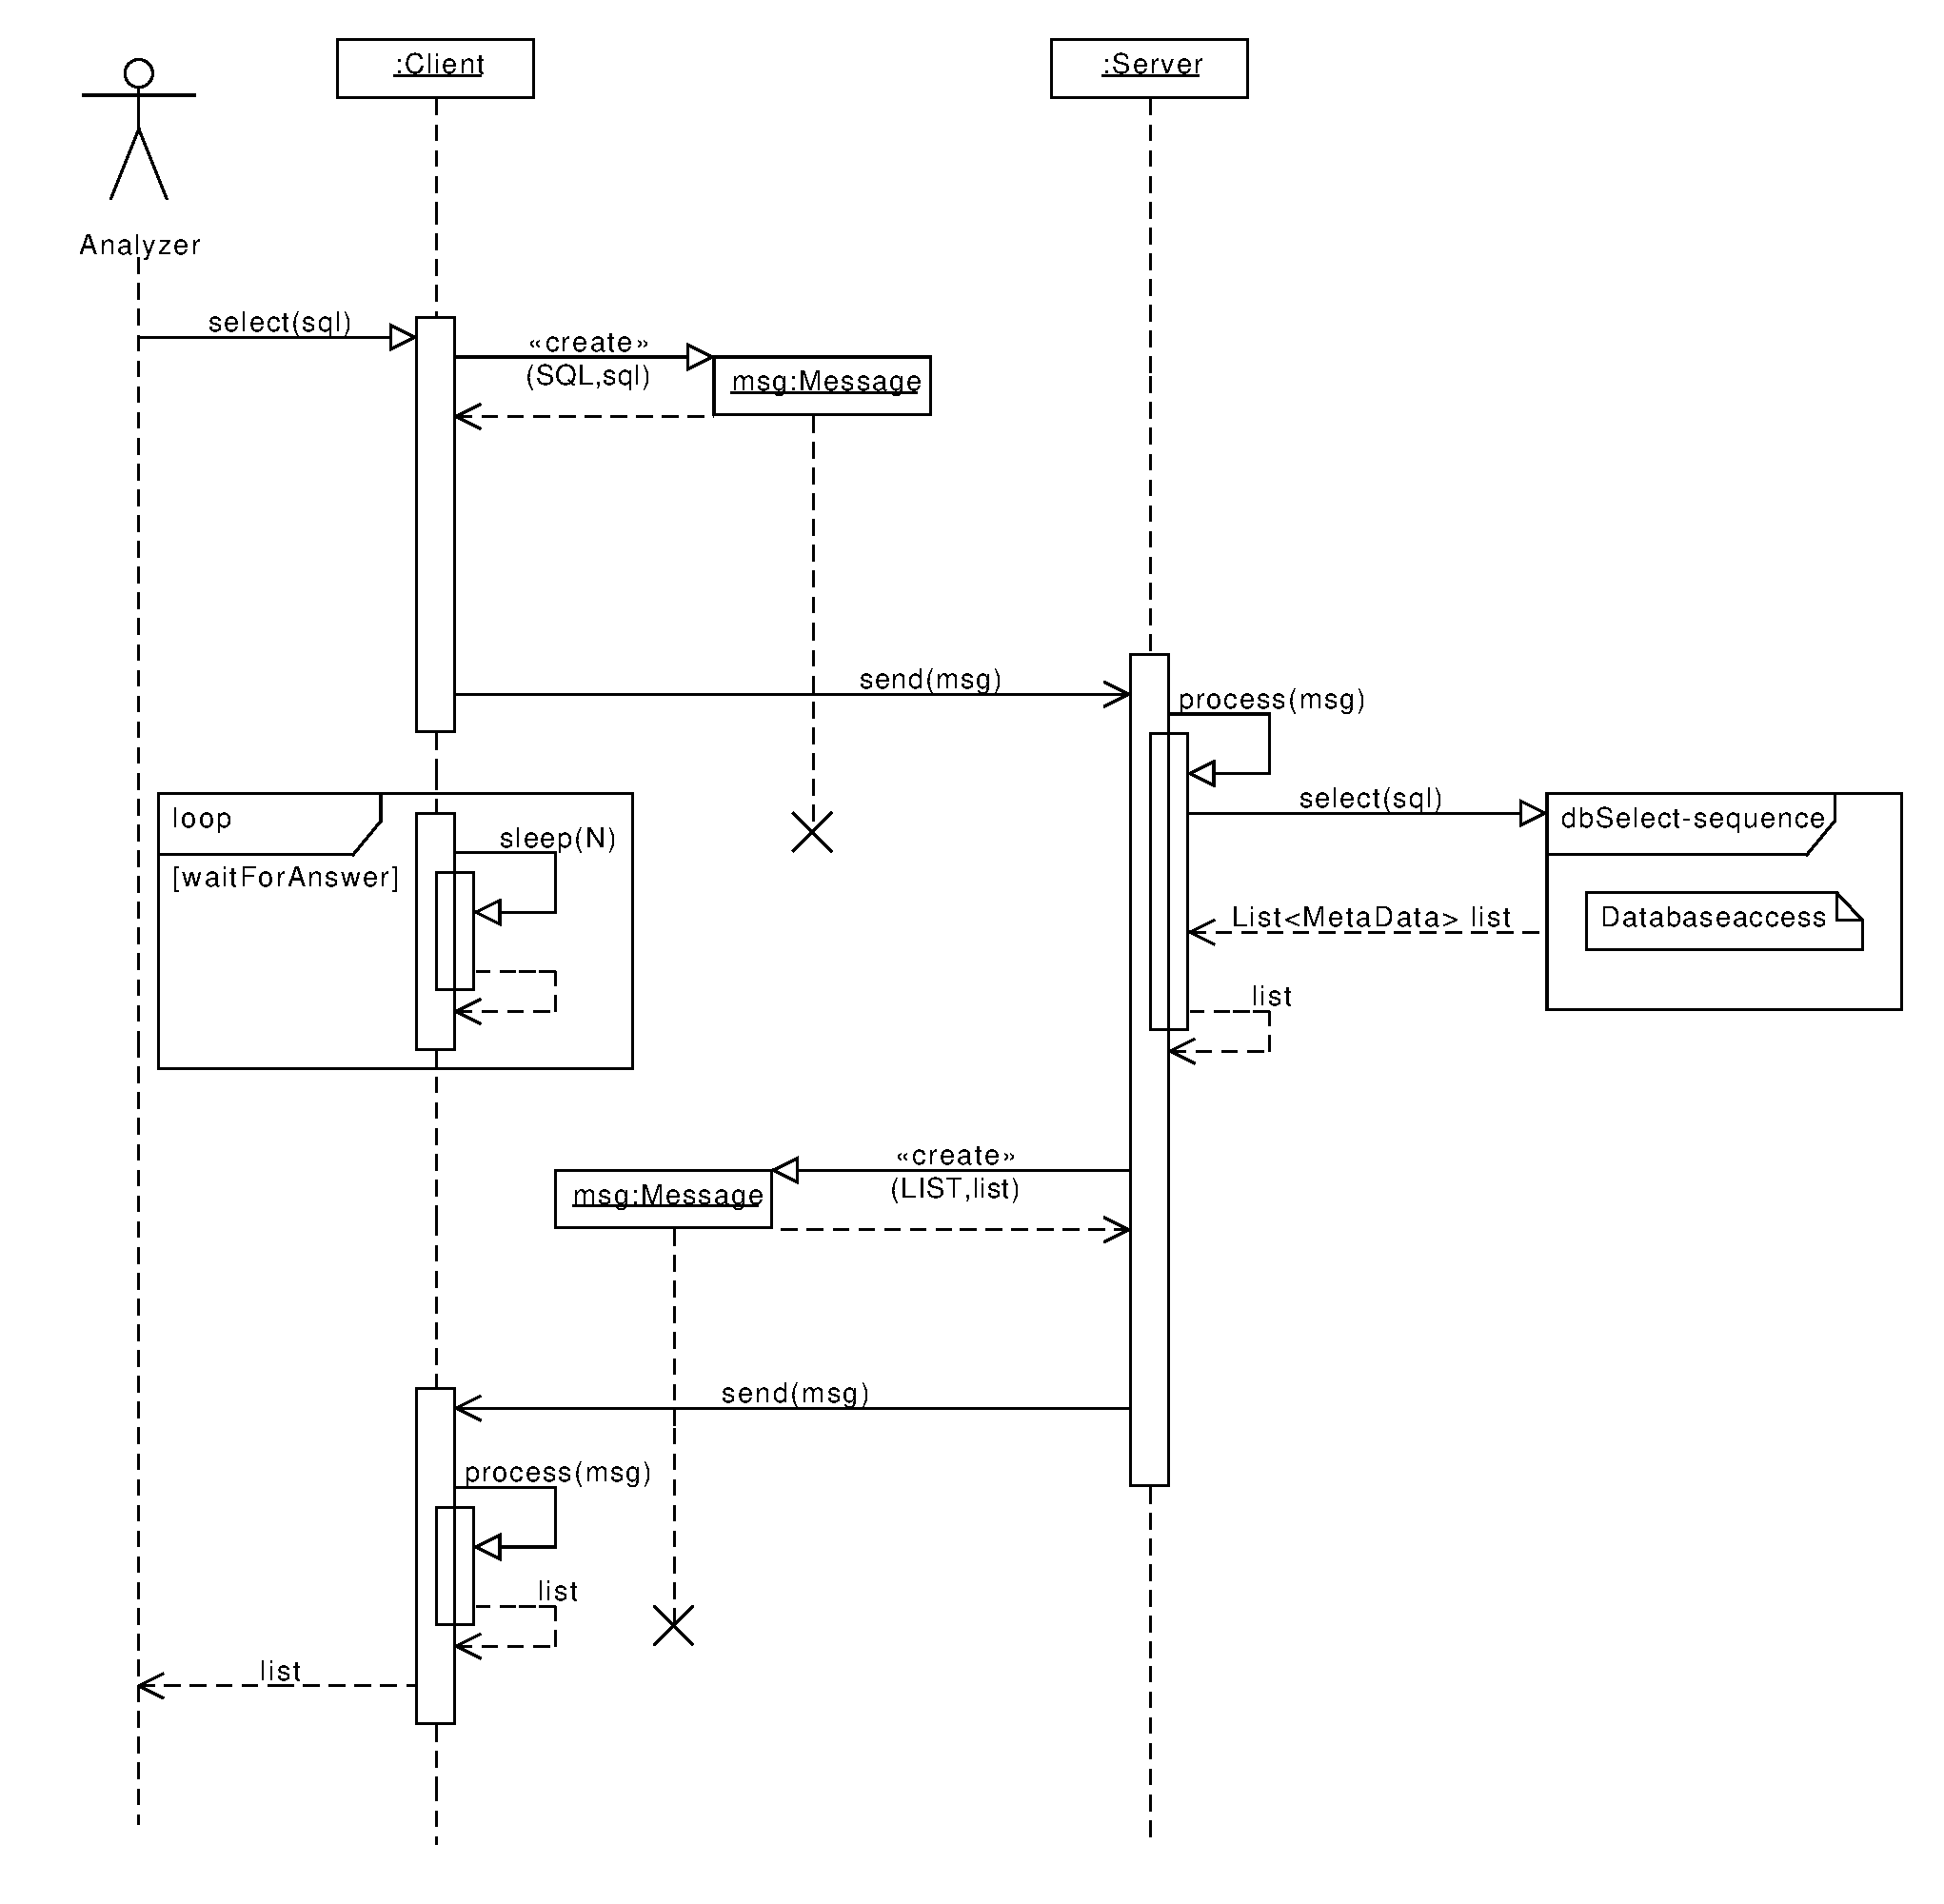
\includegraphics[width=\textwidth]{design/frontend/sequence/select-sequence.pdf}
%	\caption{Sequenzdiagramm: Select}
%\end{figure}

\subsection {add / deleteObserver}
\todo{sequence: addObserver}
%\begin{figure}[h]
%	\centering
%	\label{design:dia:sqc:select}
%	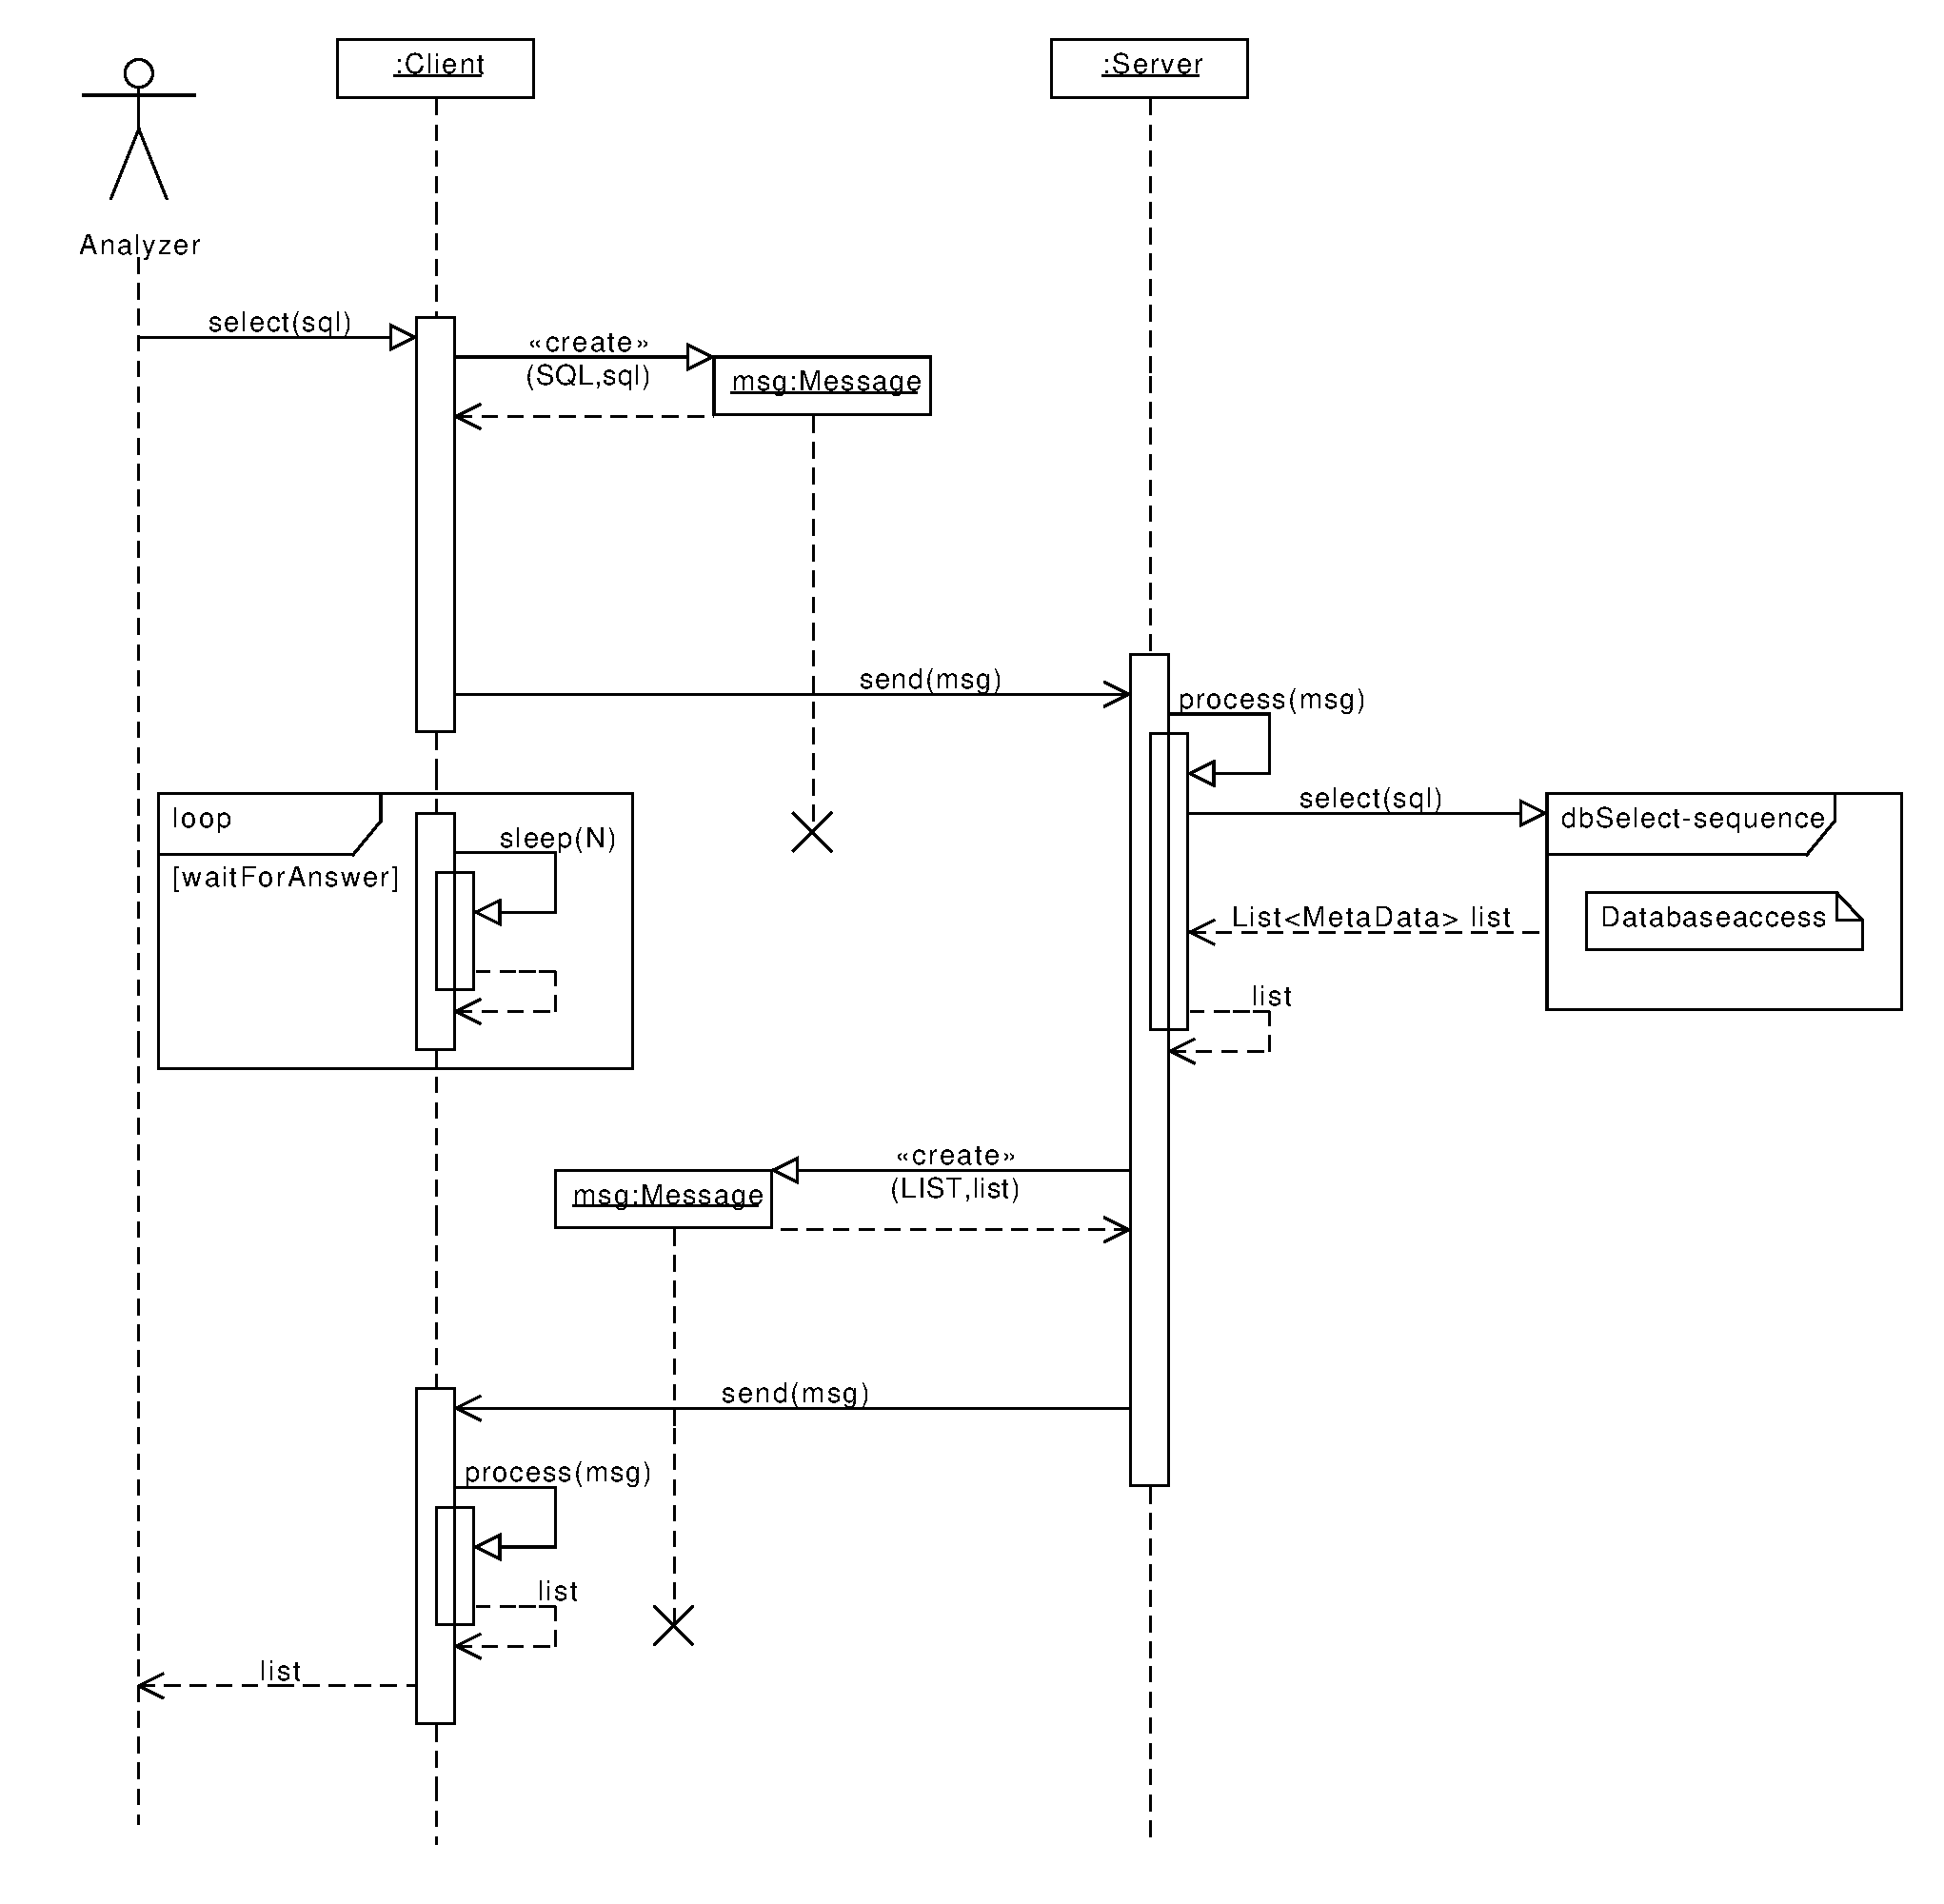
\includegraphics[width=\textwidth]{design/frontend/sequence/select-sequence.pdf}
%	\caption{Sequenzdiagramm: Select}
%\end{figure}

\subsection {notifyClients}
\todo{sequence: notifyClients}
%\begin{figure}[h]
%	\centering
%	\label{design:dia:sqc:select}
%	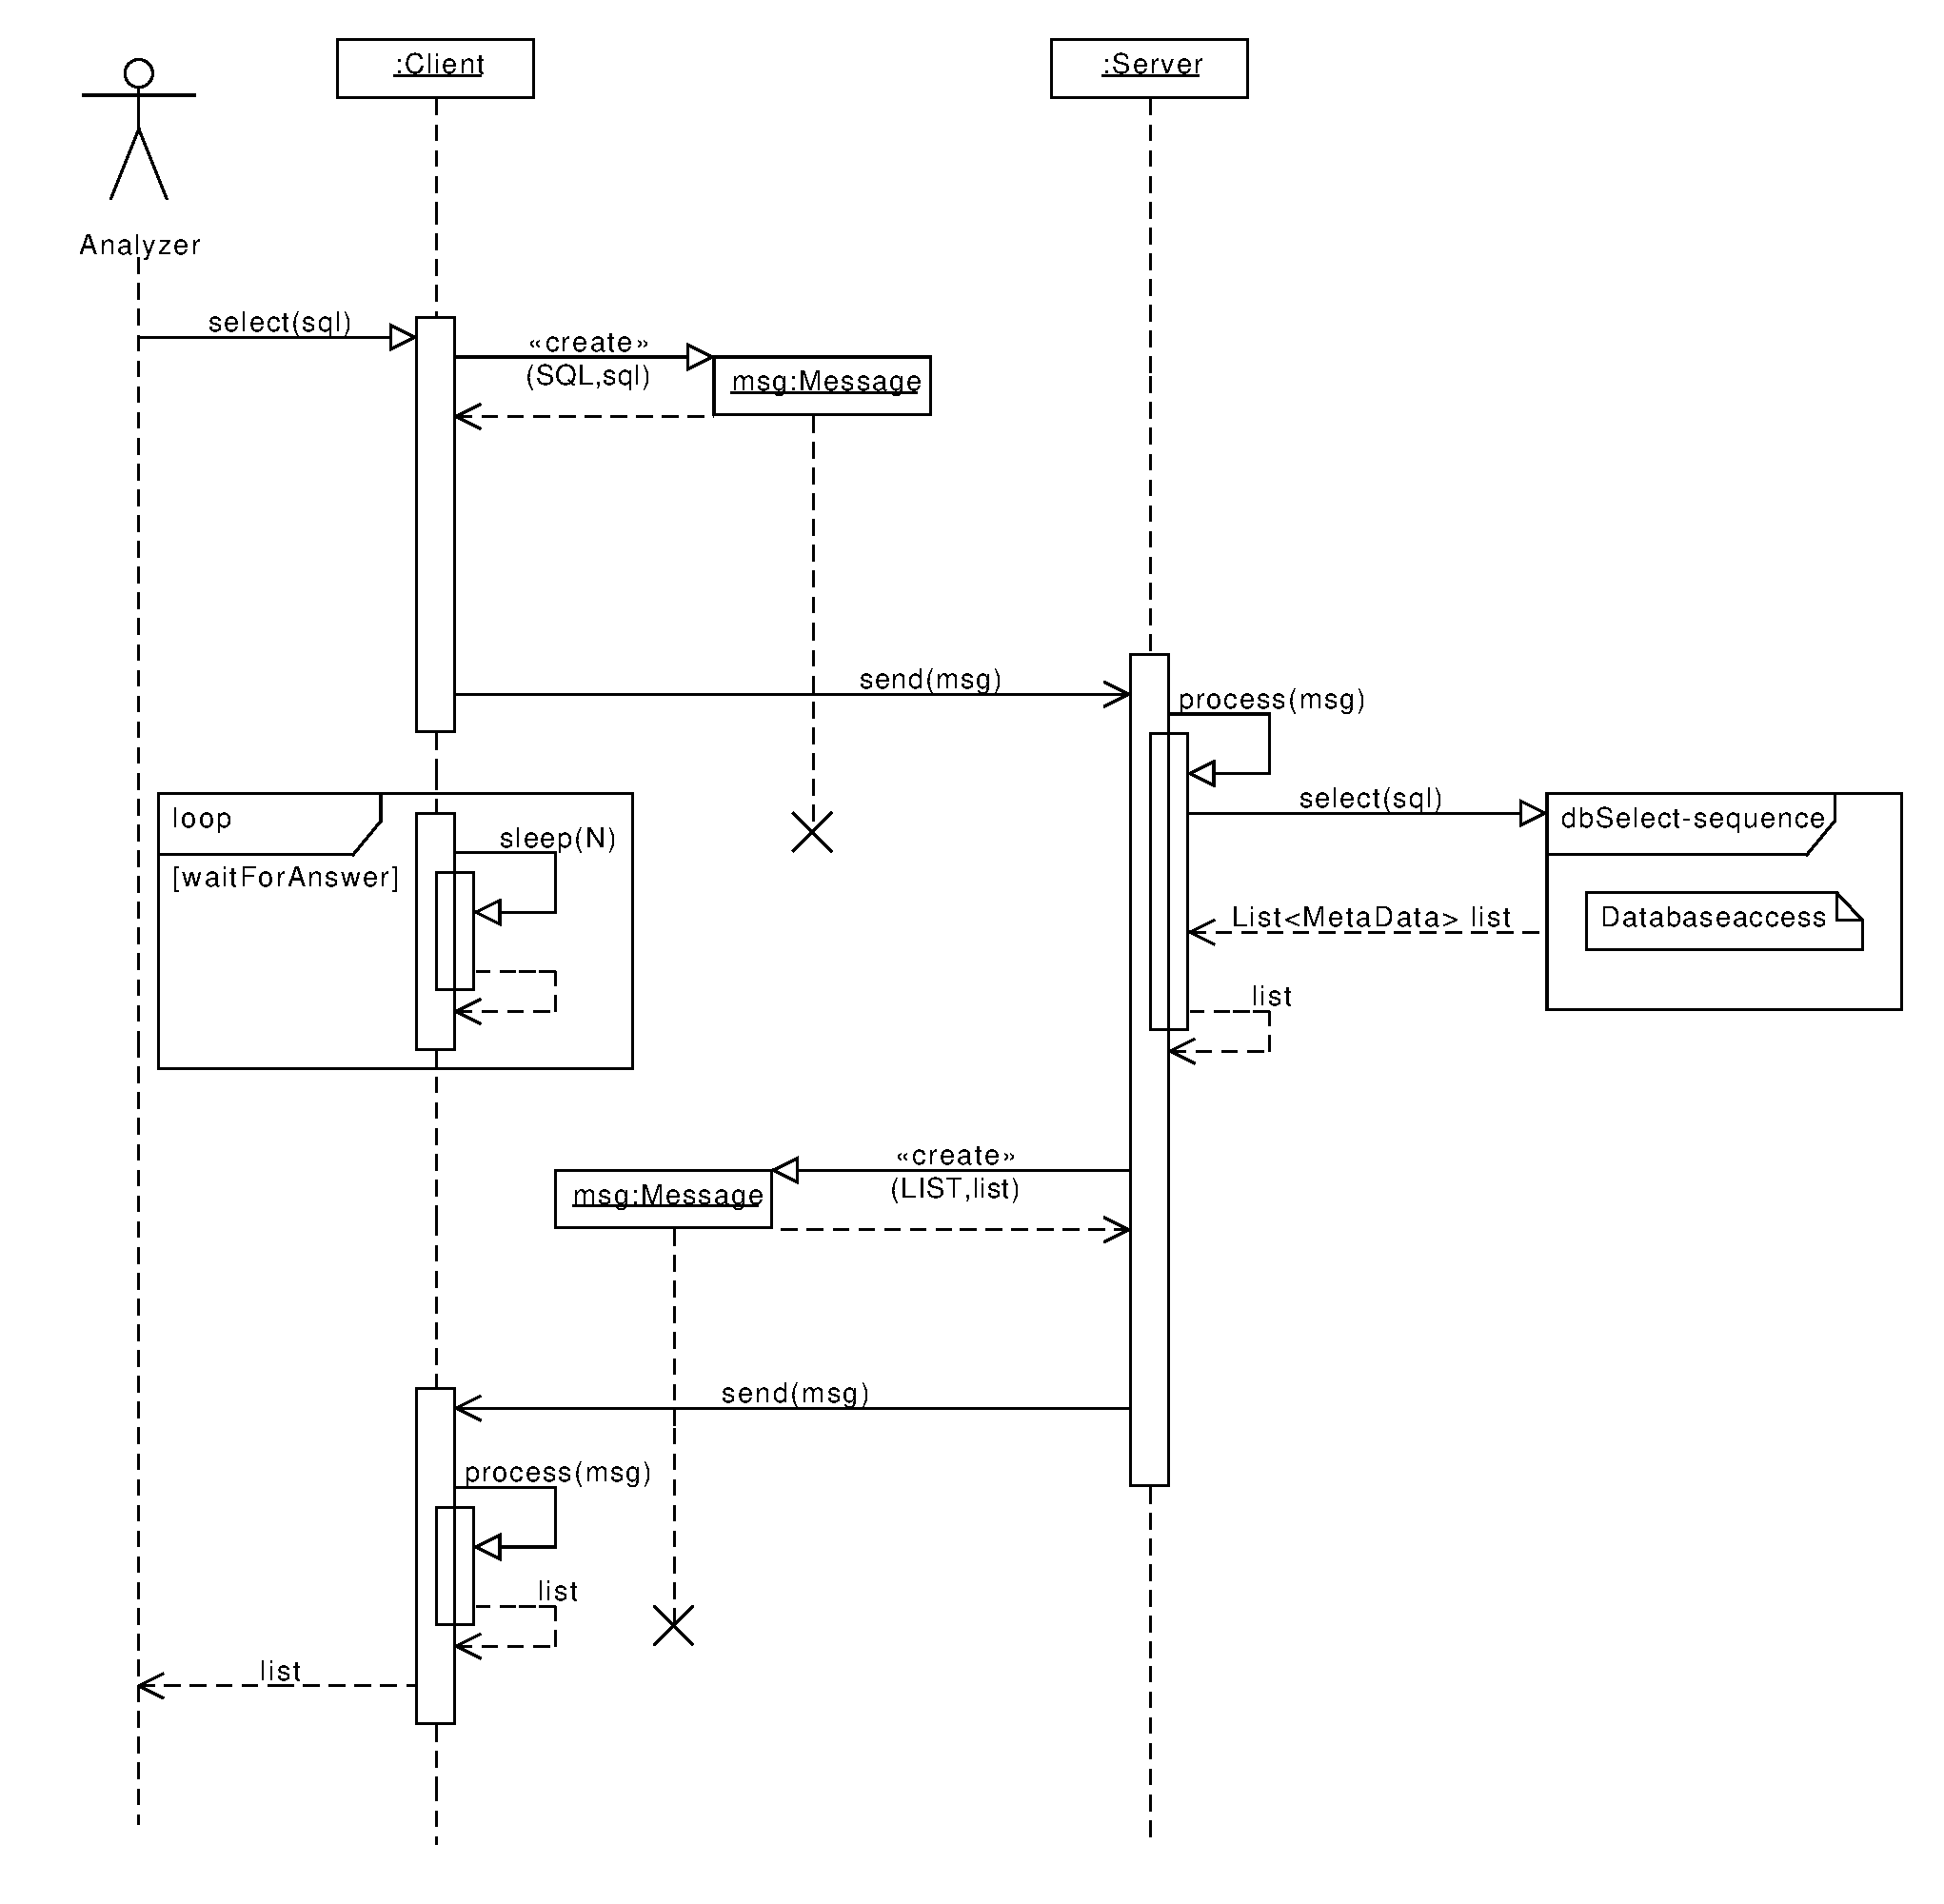
\includegraphics[width=\textwidth]{design/frontend/sequence/select-sequence.pdf}
%	\caption{Sequenzdiagramm: Select}
%\end{figure}

\section{Klassen und Komponenten}
